\documentclass{article}


\usepackage[utf8]{inputenc}
\usepackage[left=1in,right=1in,bottom=1in]{geometry}
\setlength\parindent{0pt}
\setlength{\parskip}{1em}
\setcounter{secnumdepth}{0}
\usepackage{outlines}
\usepackage{hyperref}
\usepackage{graphicx}
\graphicspath{ {imgs} }

\title{Urban Social Geography}
\author{Carla Hyenne }

\begin{document}

\maketitle

\tableofcontents

%%%%%%%%%%%%%%%%%%%%%%%%%%%%%%%%%%%%%%%%%%%%%%%%%%%%
%											LECTURE 1
%%%%%%%%%%%%%%%%%%%%%%%%%%%%%%%%%%%%%%%%%%%%%%%%%%%%

\pagebreak\section{Urban Geographical Traditions}
\date{September 27th, 2021}

Draw a general outline of how urban geography has been practiced in the last 50 years, and how it interrogates some of urban geography's main concepts and approaches.

\subsection{What is "the urban"?}

\subsubsection{Urban Age}

We are living in the Urban Age, where the population growth is proportional to urban growth. Since circa 2005, the majority (more than 50\%) lives in urban areas, or cities, as opposed to rural areas.

Urbanization is a \textbf{global phenomenon}. It started with the global North (USA, Western Europe) in the 19th century, spread to South America, USSR, Oceania in the 1950s, and Africa, Asia in the 1990s. Urbanisation intensified in the 1990s, and as of the 2000s, Asia dominates the economic growth and urbanisation.

Urbanization isn't equal throughout the world. For example, in 2018, ~40\% of Africa's population was urban, ~50\% in Asia, ~75\% in Europe, ~80\% in Latin America and North America, and ~70\% in Oceania.

\begin{center}
	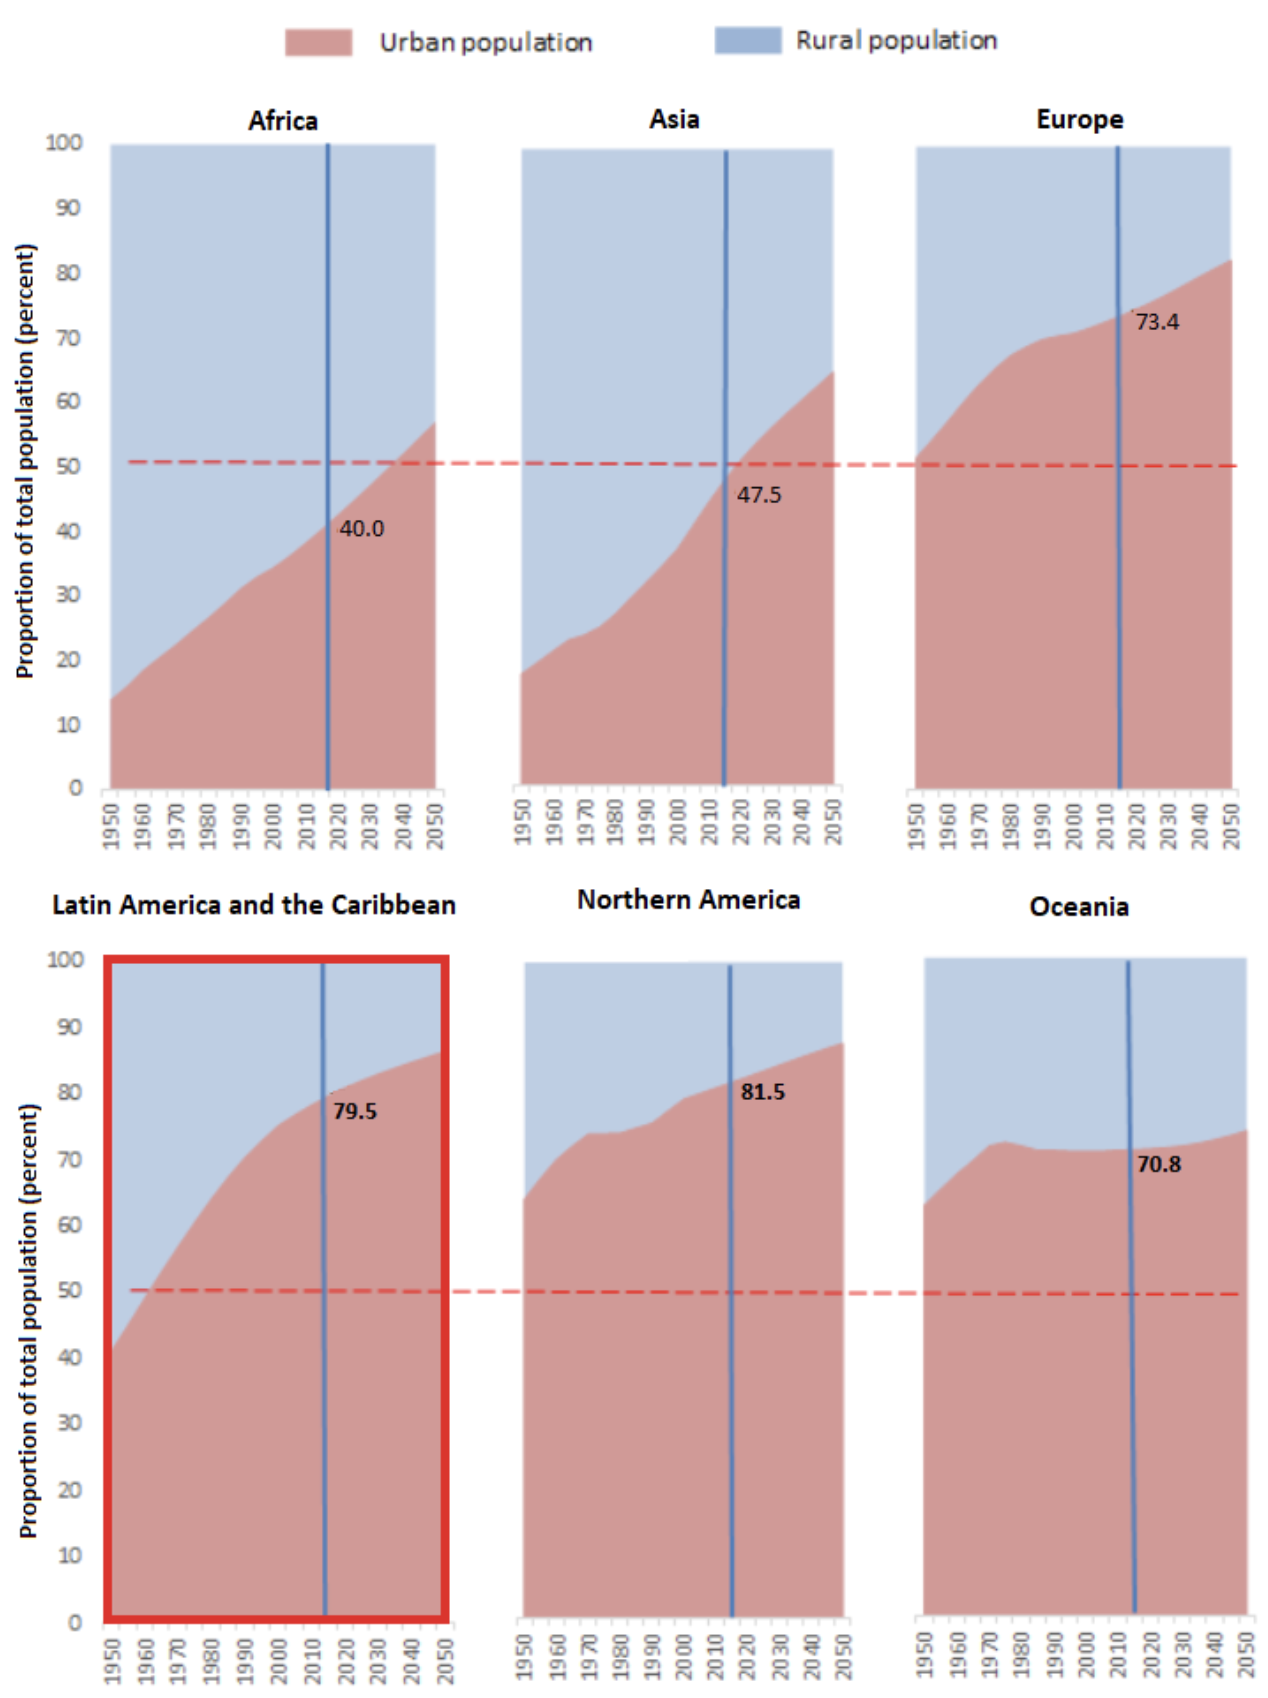
\includegraphics[width=30em]{urban_rural_proportion}
\end{center}

Is urbanization really "global"? Are we really in an "urban age"? How we measure the urban depends on statistics and national definitions and categories that diverge. It is impossible to find one definition of the urban. What is understood as "the urban" is a \textit{chaotic abstraction}, and doesn't neatly overlay cities in the spatial sense (boundaries). 

This makes the distinction of the urban vs. the rural, and the categorisation of space in either or, a black box. Is it important to think about the rural? What is difference between the urban and the city?

\subsubsection{What is the difference between the urban and the city?}

The urban is a phenomenon, a process, and elements of the urban can exist outside of the city. 
It is a set of values which direct how we might organise a city.

The city is a built environment, made of concrete. It is a marker in space, it is a physical manifestation of the urban. 
It has boundaries and is political - cities have mayors and elections, for example.

Thus, the urban is greater, theoretically, than the city.

\subsubsection{Urban Conceptualisations}

\begin{itemize}
  \item A distinctive way of life, which can take place in cities but also outside of the city (suburbs, rural, slums)
  \item It epitomises a particular society (capitalist, industrial, fordist, modern, classist...). The urban can therefore be categorised differently depending on the context and time period. 
  \item Projects symbolic power (see city conceptualisations)
\end{itemize}

\subsection{What is "the city"?}

\subsubsection{City Conceptualisations}

\begin{itemize}
  \item A lump of material, the \textbf{built environment}
  \item The non-city is... what? the rural? It is hard to say where the city ends. For examples, large boulevards connecting the city to "outside" spaces may have shops along them, which could be characteristic of the city. But are they still part of the city?
  \item A complex division of labour, with increasing efficiency and surplus, but also inequality
  \item Projects symbolic power, through skyscrapers and impressive architecture that reminds the world of the city's social/political/economic dominance. Think of the CCTV tower in Beijing, World Trade Center in NYC, Burj Khalifa in Dubai. But what is behind this image of spectacular urbanism? Is it a facade?
  \item Is administrative, with administrative boundaries
\end{itemize}

\subsection{The Urban as a Process: Urbanisation}

Urbanisation is:

\begin{enumerate}
  \item \textbf{Demographic process} in which cities gain more and a wider variety of residents, with an increased density
  \item It speaks to the increasing \textbf{globalisation of urban economic, political and cultural influence}
  \item It helps us consider \textbf{how space is organised} through processes of uneven development
\end{enumerate}

Urbanism is:

\begin{enumerate}
  \item Narrowly defined as \textbf{urban design}
  \item Gaining an \textbf{urban attribute}, a psychological and sociological feeling, giving particular meaning to urban space. \textit{Flaneurs, dandys}
\end{enumerate}

Planning is:

\begin{enumerate}
  \item A future-oriented activity, where actors of various types engage to govern how development will take place
\end{enumerate}

\subsection{What is "geography"?}

Geography is the terrain, the typologies, the interconnectedness of space and 'something' within that space; the \textbf{social and physical processes within the context of space}.

Geography is defined by "how" we study, rather than "what", with an emphasis on space. There are different concepts of space: territory, scale, place, and networks.

The \textbf{territory} defines boundaries, and sovereignty of a space (the Brussels capital has sovereignty within Belgium). 

The \textbf{scale} defines the sensitivity of processes (teaching is a small scale, commuting is a large scale, the Brussels capital scale is greater than its territory). 

The \textbf{network} defines hubs and leaks beyond the territory, towards micro-networks (Brussels connected to other cities via a transport network, but also by people living in eg. Ghent and commuting to Brussels to work. This is a leak of taxes and money from the capital to Flanders/Wallonia)

The \textbf{place} is the attachement of meaning, sentiment, to a place (how Brussels is represented in Flemish vs. Wallonia media)

\subsection{What is being "critical"?}

To be critical is to be aware of your own biases, and not cherry-picking your information. To be critical is to fact-check and question, to be reflexive about your own positionality. You should bring up new concepts, and take seriously the experience and position of others. Critical research should be socially relevant and politically engaged. The Chicago School would define it as \textit{"reducing the illusions in society itself"}.

Brenner and Schmidt are critical authors of the Urban Age.

\subsubsection{Epistemological Rules of Thumb}

\begin{enumerate}
  \item There is no universal theory of anything
  \item Every theory has birthmarks: what were the questions, situated in time and space, that gave rise to formulating a search question/theory in a particular way?
  \item Reflexivity on birthmarks is required if you want to be critical, therefore all theories need to be provincialised
  \item Can theories "speak" across contexts?
  \item Engaged pluralism might allow for inter=theoretical conversation and comparison
\end{enumerate}

\subsection{Foundational Approaches}

After WWII, geography moved from purely territorial to plural definitions, from regional (urban) geography (descriptive, map-oriented, idiographic) to a spacial science (nomothetic, method-driven, applied orientation).

The \textbf{materialist approach} has materialist frameworks, is concerned with distribution and social-justice, and agenda-setting: Marxist geography, Structuralist geography, Critical geography, Radical geography, Feminist geography, Critical realist geography

The \textbf{humanistic approach} is about the experienced city, issues of representation and discourse, uses qualitative methods, and is about giving voice: Humanist geography, Cultural urban geography, Post-structuralist geography, Post-colonial geography, Queer geography

%%%%%%%%%%%%%%%%%%%%%%%%%%%%%%%%%%%%%%%%%%%%%%%%%%%%
%											LECTURE 2
%%%%%%%%%%%%%%%%%%%%%%%%%%%%%%%%%%%%%%%%%%%%%%%%%%%%

\pagebreak\section{Theories of world-city formation}
\date{Octobre 4th, 2021}

The first session on world and global cities aims to:
\begin{itemize}
  \item Provide a framework to conceptualise and analyse cities under (economic) globalisation
  \item Give an overview of key theories of world-city formation dating back to the 1970s-1980s and onwards
  \item Introduce model-based approaches to the world-city network as a heuristic to map out how cities are positioned on global flows of capital, knowledge, and people
  \item Discuss a number of key critiques of the alleged "world/global cities paradigm", voiced from social constructivist and post-colonial positions
\end{itemize}

\subsection{Centrality of cities/city-regions in the global economy: Friedmann, Sassen, Scott}

How are cities central in the global economy? What does it mean to say that cities are powerful? 

\begin{outline}
	\1 Concentration of businesses, seats of corporate power, migration of elites to the city
	\1 Cities are administrative and political authorities
	\1 The city is a hub of ideas, culture, social influence, and knowledge transfer
	\1 Flows converge in cities, and flow between big cities: it's easier and faster to travel between cities than from a city to its periphery or towns. The substance of the flows can be knowledge, people, capital, commodities
\end{outline}

The five most powerful regions of Europe are Deltametropolis, Flemish Diamond, RheinRuhr Area, Ile-de-France, and Greater London.
There are multiple ways that we can measure the power, or influence, of such world-cities:

\begin{outline}
	\1 \textbf{Weight of area in national context}: the \textbf{GDP} is higher, and the density of population is higher\footnote{Higher than the European and national averages. This applies to the rest of the indicators.}
	\1 \textbf{Patents}: number of patents is higher. This indicates the level of social and technological innovations of a city
	\1 \textbf{Education}: the proportion of people educated at a high level is higher. This indicates a different labour market structure
	\1 \textbf{Employment by sector}: proportion of employment in services is higher, and proportion of employment in industry or agriculture is lower
\end{outline}

\subsubsection{John Friedmann, \textit{World City Hypothesis}}

\textit{tldr; global cities are basing points in a global (economic) urban system, organising and articulating production and markets}

\textbf{Why are cities economically central and powerful?}

There were predictions in the 1980s that ``the end of the city" was coming, due to ICT and cheap mass transportation. Instead, these gave rise to new forms of uneven development related to \textbf{functional centrality} on a more global scale. People could travel from further distances and still work in the functional (city) centre, and have relationships with people from a longer distance.

World cities were inserted in a \textbf{global urban system}, in which urban processes that cross-cut national and regional borders are conceptualised: this insertion drives structural change in cities and renders some places powerful. We have to look beyond national urban systems, and start thinking about processes of \textbf{globalisation}, ie. on a global scale. A great part of economics became international, and only the global urban system can explain what is happening internationally. 

In this sense, world-cities are the base points to explain ``spatial organisation and articulation of production and markets'' (\textit{The World City Hypothesis}, Friedmann, 1986), ie. the geo-economic restructuring of the world.

There is a new \textbf{international division of labour} in the world. Companies offshore their production activities or relocate to (semi) peripheries to drive prices down because of cheaper labour markets, in order to stay competitive. There are new actors, TNCs and MNCs (trans- and multi- national corporations) that dominate and organise a global supply chain that is highly integrated\footnote{This complex, interconnected division of labour is illustrated by 1) the Evergreen container ship that blocked the Suez canal and blocked distribution of goods for a week, or 2) the lack of bicycles during the covid pandemic, when manufacturing plants had to close due to regional or national safety measures.} Given the importance of TNC/MNCs, mapping their headquarters can be used to locate world-cities. 

This illustrates that world-cities are sites for centralised \textbf{command and control} functions in a complex global economy. It implies a hierarchy connecting the core and the periphery, with core cities absorbing the surplus (and thus getting richer and growing in all dimensions)\footnote{This means that locations and cities will benefit unequally from this geography: the US (Global  North) producing in Argentina (Global South) will benefit the US, who extracts the profit, and disadvantage Argentina, who has a cheaper labour market}. But, (semi) peripheries can still hold local command and control functions.

\subsubsection{Sassen, \textit{The Global City}}

\textit{tldr; global cities are cities where APS (Advanced Producer Services) are produced for the international market; APS have control capabilities over global production, and they produce global financial markets}

Sassen writes at the same time as Friedmann, in a context of de-industrialisaiton (specially in NY, London, Tokyo) and fiscal crisis of the local state, and cities are trying to figure out what they might become.
Sassen focuses on the \textbf{shift to service economies}, especially finance services and auxiliary services in law, management consultancy, accounting, auditing, advertising, etc. These auxiliary services are called \textbf{advanced producer services (APS)}, they are not producing consumable goods, but rather goods that are consumed as they are produces (eg. legal advice).

Advanced producer services are embedded in global cities, and they have \textbf{control capabilities} to manage global production and produce global financial markets. There is a \textbf{labour market polarisation}, with high and low skilled labour forces surround APS, which results in the ``peripheralisation'' of the core (eg. sweatshops).

Sassen says that \textit{``global cities are sites for the production of specialised services needed by complex organisations for running a spatially dispersed network of factories, offices, and service outlets; and the production of financial innovations and the making of markets, both central to the internationalisation and expansion of the financial industry''}.

Global cities are connecting to the world of finance for investments, and growing the need for concentration and control. This geography is self reinforcing.

Why are APS concentrating in a limited number of cities? There are several interlocking \textbf{path dependencies}:
\begin{outline}
	\1 \textbf{Large services market}: there is access to firm/client relations, for out-sourced APS
	\1 \textbf{Labour market and associated culture}: a cosmopolitan elite and `yuppie' (young urban professional) culture is formed, since the 1980s
	\1 The most specialised and globalised APS firms need \textbf{synergies} with similar firms in the city, which creates an \textbf{APS complex}. For example, financial firms, ICT firms, advertising, management consultancy, accountancy, and legal services all need each other to some extent
	\1 The APS complex produces \textbf{cross-border connections} through a network of affiliates and other partnerships
\end{outline}

Even within the city, there are APS clusters. For example, the concentration of law firms in Avenue Louise and in the EU quarters of Brussels.

\subsection{Scott, \textit{Global City Regions}}

\textit{tldr; global city-regions are a complex assemble of cities/settlements/hinterlands that are interconnected via production networks, themselves oriented towards global economy}

Sassen's views of global cities as APS centres fits London, Hong Kong, Brussels, etc., but there are large-scale territorial entities like the Pearl River Delta\footnote{One of the most densely populated urban regions of the world, considered a megacity, and one of the wealthiest regions in China.} and the Bay Area, which have global power but are not cities. Many production processes don't need an `urban core'.

The need for centrality is applicable to \textbf{post-Fordist modes of production\footnote{Post-fordism is the idea that modern industrial production has moved away from mass production in huge factories, towards specialised markets based on small flexible manufacturing units}, where knowledge is central}. The concentration is a by-product of globalisation and technological innovations (cf. cognitive-cultural capitalism). 

So, not only APS need to be centralised. For knowledges that are not easy to de-centralise, proximity matters. For example 1) industries in which it is important to communicate with clients face-to-face, or 2) tailored, just-in-time delivery. Concentrating an activity in one area also makes it easier to receive federal/public investments (ie. investments drive centralisation).

\textbf{Global city-regions} are a complex ensemble of cities/settlements/hinterlands, that are interconnected via multiple production networks, which in themselves are oriented towards the global economy. APS firms can still be used as a general indicator of the globalisation of Global City-Regions, as they produce the tools to enable proper functioning in a global economy.

\subsection{Mapping world city networks}

Comparing the importance of urban connections (eg. London/Hong Kong vs Paris/Tokyo) is difficult when using available data sources, and without using a secondary data source or creating new data.
This is because there is a research gap regarding world-city networks.
Secondary data could be information on inter-city transportation or information flows (eg. flows of airline passengers). New data collections could be developing a methodology to use specific attribute data to assess inter-city relations (eg, the GaWC-heuristic).

Are airline flows a good way to measure global economic influence, and thus helpful to map the world-city network?
\begin{outline}
	\1 Some cities which are not global-cities have airports, and maybe vice versa
	\1 People travel for leisure, which may tell us something about the local economy but not about the influence of the city's economy on a global scale
	\1 A lot of goods are moved by other means than air, eg. water or land
\end{outline}

Therefore, we need a \textbf{new metageography} of spaces of flows. This would be a new socio-spatial structure.

The GaWC (Globalisation and World Cities) heuristic is an example of a new way to gather data\footnote{See \url{https://www.lboro.ac.uk/gawc}}. The starting point is the presence of international APS firms, that is used as a general indicator for command and control functions of cities. Since APS firms have office networks that comprise of the most important cities in the global economy, we make the core assumption that inter-city relations can be assessed based on the APS firms being present in multiple cities. $\rightarrow$ we measure the connectivity of cities.

APS don't represent all of the global economics, but they represent strategies of the command-and-control of APS firms. 

\subsection{Critiques and complementary views}

The GaWC heuristic is a powerful tool to map and spatially analyse the global connections of world/global cities, but has been criticised from various angles: post-colonial, social-constructivist, political-economy, and financialisation perspectives.


\begin{outline}
	\1 \textbf{Post-colonial critique}: there is a western bias in the knowledge production of urbanisation, people are dropped off the map of urban studies research. 
		\2 Off the geographical map refers to (world) cities in the Global South
		\2 Off the conceptual map refers to the focus on a limited number of economic processes, and ignoring equally important inter-urban connections
		\2 World cities research ignored the role and position of `ordinary' cities in the global economy,  or reads them in light of Eurocentric global city theories 
		\2 Tendency in urban studies to reject world/global city theory as only befitting the Global North, but not on the basis of a sound argumentation: non-representation as a `result', not a `neglect'
	\1 \textbf{Social-constructivist critique}: stresses the political natural of world-city formation and its often un-debated consequences
		\2 Post-modern knowledge theory: world cities are not a `given' but a product of global and local forces, and crucially mediated by acts of representation
	\1 \textbf{Financialisation}: GaWC heuristic is a powerful shorthand for the geographies of world/global cities, but world-city functions are often assumed instead of researched 
		\2 etc...		
\end{outline}

\subsection{Key words}

World cities
World city-regions
Global urban system, global economic system
GaWC
Command-and-control function of cities

%%%%%%%%%%%%%%%%%%%%%%%%%%%%%%%%%%%%%%%%%%%%%%%%%%%%
%											LECTURE 3
%%%%%%%%%%%%%%%%%%%%%%%%%%%%%%%%%%%%%%%%%%%%%%%%%%%%

\pagebreak\section{Polarisation in World/Global Cities}

This second session on world and global cities discussions the connections between the positionality of cities on global circuits of value and their internal social and economic structure:
\begin{itemize}
  \item Applies Harvey's framework to analyse urban  entrepreneurial export-base enhancing strategies
  \item Focuses on the polarisation debate, which has centred on the mechanisms that produce income \& professional divides, the contextual factors that mediate such polarisation processes, the role of high/low-skilled migration, gentrification, etc.
\end{itemize}

\url{https://www.youtube.com/watch?v=qOP2V_np2c0&ab_channel=RSA}

\subsection{Polarisation}

\textit{tldr; polarisation is a class division that is reproduced through space, and is stronger in global cities}

Income disparity looks different in different cities. Chicago, Detroit, LA, Miami, New Orleans, SF, NYC, all have different, contextual landscapes of polarisation.

Polarisation is the reality of \textbf{class division}. \url{https://www.opportunityatlas.org} is an income map that traces neighbourhood effects, based on census data. The \textbf{neighbourhood effect} is the idea that where you are born, predetermines your life. This is due to the amenities, infrastructure, opportunities associated to the geographical location.

Polarisation is one of the starting point of debates in global cities: it raises the questions about \textbf{how class divisions in cities are reproduced in/through space, but also why there is a deep polarisation in key nodes in the global economy}, ie. in world/global cities.

Picture LA, a `citadel' city where polarisation/segregation are both horizontal and vertical (there are no wealthy people residing on the ground floor). Wall Street in LA is a poor neighbourhood in decline, or a `zone in transition', yet it is contrasted with nice hotels. This says to people that `those who have nothing to do here, should not be here'.

\subsubsection{New York City}

We can see how NYC's polarisation patterns have evolved in the last decade, since the 2008 recession: \textbf{polarisation and income distribution gaps have increased}. 

The median family income has fallen\footnote{Income can be equated to labour}, and the decline in income is steeper in NYC than in the state of NY. The share of total income going to the top 1\% continues to increase (it only declines during a financial crisis but quickly rebounds), such that the top 1\% own over 40\% of the total income and the income of the lowest household is \texttildelow17.5\% of the top earners' income. And the gap in increasing.

\textbf{Productivity has increased but wages have not}: for 1 hour of work, an extra 14\% is produced, but the wages have not proportionally increased. The profit is not going to the workers, and a full-time worker at a minimum wage now lives under the \textbf{poverty line}.

\begin{center}
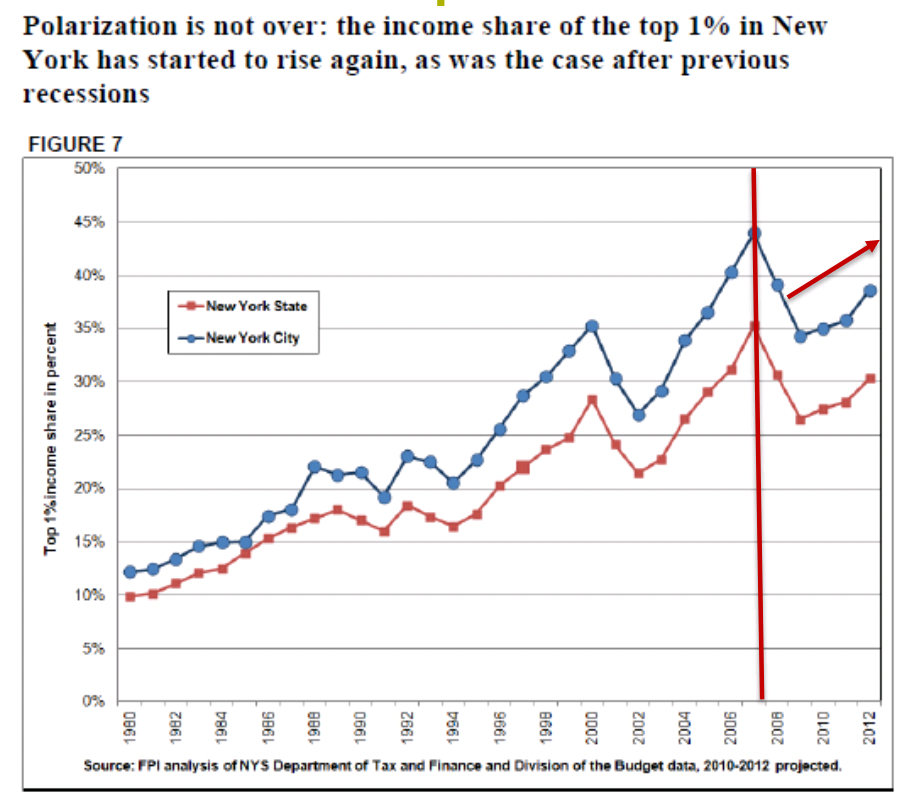
\includegraphics[width=23em]{nyc_income_gap}
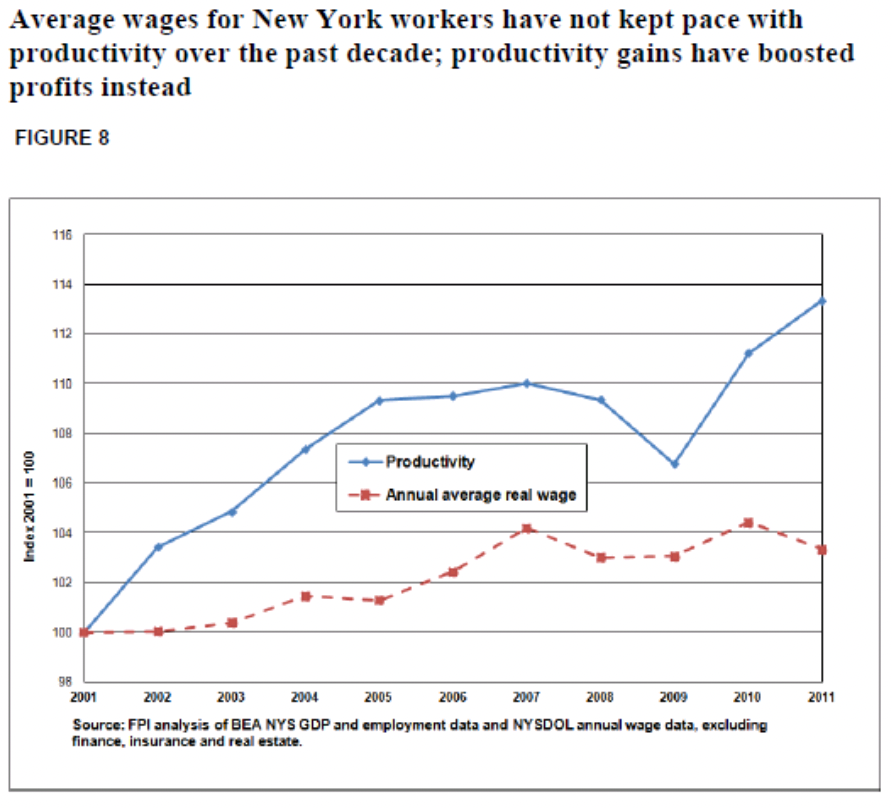
\includegraphics[width=23em]{nyc_productivity_gap}
\end{center}

Why is it that world/global cities have become so polarised?


\subsection{Conceptualisation}

\subsubsection{}


\subsection{Polarisation thesis}

\subsection{Criticism}



%%%%%%%%%%%%%%%%%%%%%%%%%%%%%%%%%%%%%%%%%%%%%%%%%%%%
%											LECTURE 4
%%%%%%%%%%%%%%%%%%%%%%%%%%%%%%%%%%%%%%%%%%%%%%%%%%%%

\section{Urban segregation: patterns and causes}

%%%%%%%%%%%%%%%%%%%%%%%%%%%%%%%%%%%%%%%%%%%%%%%%%%%%
%											LECTURE 5
%%%%%%%%%%%%%%%%%%%%%%%%%%%%%%%%%%%%%%%%%%%%%%%%%%%%

\section{Neighbourhood effects and living with diversity}

%%%%%%%%%%%%%%%%%%%%%%%%%%%%%%%%%%%%%%%%%%%%%%%%%%%%
%											LECTURE 6
%%%%%%%%%%%%%%%%%%%%%%%%%%%%%%%%%%%%%%%%%%%%%%%%%%%%

\section{Cultures of urban research}

%%%%%%%%%%%%%%%%%%%%%%%%%%%%%%%%%%%%%%%%%%%%%%%%%%%%
%											LECTURE 7
%%%%%%%%%%%%%%%%%%%%%%%%%%%%%%%%%%%%%%%%%%%%%%%%%%%%

\section{Urban cultures}

%%%%%%%%%%%%%%%%%%%%%%%%%%%%%%%%%%%%%%%%%%%%%%%%%%%%
%											LECTURE 8
%%%%%%%%%%%%%%%%%%%%%%%%%%%%%%%%%%%%%%%%%%%%%%%%%%%%

\section{Transport and cities: a historical hegemony}

%%%%%%%%%%%%%%%%%%%%%%%%%%%%%%%%%%%%%%%%%%%%%%%%%%%%
%											LECTURE 9
%%%%%%%%%%%%%%%%%%%%%%%%%%%%%%%%%%%%%%%%%%%%%%%%%%%%

\section{Critical perspectives on urban transport}

%%%%%%%%%%%%%%%%%%%%%%%%%%%%%%%%%%%%%%%%%%%%%%%%%%%%
%											READINGS
%%%%%%%%%%%%%%%%%%%%%%%%%%%%%%%%%%%%%%%%%%%%%%%%%%%%

\section{Readings}

\subsection{Polarisation in World/Global Cities}

\subsubsection{Hamnett, \textit{The changing social structure of global cities: Professionalisation, proletarianisation or polarisation}}

\begin{outline}
	\1 There are three trends studied: professionalisation, proletarianisation and polarisation. These concepts have shaped the social structure of global cities, and the paper aims to understand whether there is a dominant trend
	\1 \textbf{Professionalisation} refers to an increase in ``professionalised'' occupations, with an increase in professional, managerial and technical workers, some on high income. Professionalisation started as a result of changes in the industrial structure (from industrialisation to a post-industrialisation era starting in the 1970s).
	\1 \textbf{Proletarianisation} is the increase in de-skilled jobs, as a result of changing industrial structures (basically the opposite of professionalisation, as a result of industrial structure changes).
	\1 \textbf{Polarisation} is the growing gap between the top and bottom ends of the occupational and income distribution, where the middle in shrinking.
	\1 Society went from a pre-industrial (pre-1840s), to industrial (1840s) and \textbf{post-industrial society} (PIS, 1970s). 
		\2 It shifted from a society dominated by manufacturing employment, to one dominated by the service sector and drastic decrease in manufacturing employment. PIS could be expected to give rise to de-proletarianisation (decline in working class) due to machinery and innovation replacing manual labour. On the other hand, capitalism generates technical innovation that could replace high-skilled labour, which would increase proletarianisation.
		\2 Researching the class structure of PIS shows that there is an upwards shift towards professionalisation, and that society is biased towards high-skilled labour (top and middle classes) rather than low-skilled (bottom class). Children with working-class parents and grandparents are now likely to be graduates and work in professional careers
		\2 However, the growth of professionalisation, and thus of the professional and managerial class, has been accompanied by an increase in income inequality and precarious work $\rightarrow$ polarisation
 \end{outline}

\subsubsection{May et. al, \textit{Keeping London Working: global cities, the British state and London's new migration division of labour}}

\begin{outline}
	\1 Instead of focusing on professionalisation and jobs at the top end of the market, this paper focuses on the bottom end and specifically on the character and composition of the people who work there (mostly  foreign-born and migrant labour). 
	It explores how state welfare, labour market, and migration policies have changed the labour market and increased the low-skilled labour demand, which is disproportionally taken up by foreign-born workers and new migrants.
	\1 It criticises Hamnett's work, saying that it focuses too much on professionalisation rather than polarisation
	\1 Regarding the state welfare policies, it did not protect wages or working conditions. Instead, Conservative governments tried hard to secure a competitive economic advantage for Britain by labour market de-regulation and welfare restructuring. The British state actively tried to facilitate the recruitment of migrant labour, at the same time restricting people's welfare.
		\2 A significant proportion of the bottom of the labour force are migrants, working long and unsociable hours, for extremely low rates, without protection offered to native workers like the benefits system
	\1 Bottom-up initiatives, and places of faith have taken on the role of campaigning for worker's rights s
\end{outline}

%%%%%%%%%%%%%%%%%%%%%%%%%%%%%%%%%%%%%%%%%%%%%%%%%%%%
%											EXAM etc.
%%%%%%%%%%%%%%%%%%%%%%%%%%%%%%%%%%%%%%%%%%%%%%%%%%%%

\section{Exam}

\href{https://bakexamenwiki.wordpress.com/urban-geography/?fbclid=IwAR1qxA_V_G9I3NVC_17dFMUmEMLisoLB-XfgdqZmQNxIsUydvhO_ZnCOFVU}{2021 Exam Questions}





\begin{outline}
	\1
\end{outline}














\end{document}